%\documentclass[11pt,a4paper]{book}
\documentclass[a4paper]{memoir}
%\documentclass{memoir}

\usepackage{titling}
\usepackage[utf8]{inputenc}
\usepackage[english]{babel}
\usepackage{mathtools}
\usepackage{hyperref}
\usepackage{booktabs}
\usepackage{amsmath}
\usepackage{caption}
\usepackage{subcaption}
\usepackage{xcolor}
\usepackage[]{rotating}
\usepackage[]{titlesec}
\usepackage[absolute]{textpos}
\usepackage{algorithm}
\usepackage{algpseudocode}
\usepackage[backend=bibtex, style=nature]{biblatex}
%\usepackage[thinlines]{easytable}
\usepackage[export]{adjustbox}
\usepackage{graphicx}
\usepackage{wrapfig}

\addbibresource{report-bibliography.bib}
\addbibresource{neuronal.bib}
\addbibresource{vision.bib}
\addbibresource{neuromorphic.bib}
\addbibresource{slam.bib}
\addbibresource{cam2spikes.bib}

%\addbibresource{report-bibliography.bib,neuronal.bib,vision.bib,neruomorphic.bib,slam.bib,cam2spikes.bib}


% Title Page
\title{SpiNNaker-based implementation of visual systems}
\author{Garibaldi~Pineda~García \\ Supervisor: Steve~Furber Co-supervisor: Dave~Lester}
\date{}

\definecolor{themecolor}{RGB}{80, 0, 127} %manchester
\definecolor{themecolordark}{RGB}{64, 26, 86} %dark-manchester
\definecolor{darkgray}{gray}{0.15}


\hypersetup{ 
%  colorlinks   = true,
%  citecolor    = gray,
%  linkcolor    = themecolordark,
%  linkbordercolor = gray,
%  citebordercolor = gray,
  allbordercolors = themecolor,
  pdfborderstyle={/S/U/W 1}
}



\graphicspath{{./images/}}



\setlrmarginsandblock{4cm}{2.5cm}{*}
\setulmarginsandblock{3cm}{3.5cm}{*}
\checkandfixthelayout
%\setlength{\evensidemargin}{\oddsidemargin}

%\makeatletter
\makechapterstyle{myVeelo}{%
  %\chapterstyle{default}
  \setlength{\afterchapskip}{180pt}
%  \setlength{\beforechapskip}{0pt}
  \renewcommand*{\chapterheadstart}{\vspace*{30pt}}
  \renewcommand*{\afterchapternum}{\par\nobreak\vskip 25pt}
  \renewcommand*{\chapnamefont}{\normalfont\LARGE\flushright}
  \renewcommand*{\chapnumfont}{\normalfont\HUGE}
  \renewcommand*{\chaptitlefont}{\normalfont\HUGE\bfseries\flushright}
  \renewcommand*{\printchaptername}{%
    \chapnamefont\MakeTextUppercase{Chapter}}
  \renewcommand*{\chapternamenum}{}
  \setlength{\beforechapskip}{18mm}%  \numberheight
  \setlength{\midchapskip}{\paperwidth}% \barlength
  \addtolength{\midchapskip}{-\textwidth}
  \addtolength{\midchapskip}{-\spinemargin}
  \renewcommand*{\printchapternum}{%
    \makebox[0pt][l]{%
      \hspace{.8em}%
      \resizebox{!}{\beforechapskip}{\chapnumfont \thechapter}%
      \hspace{.8em}%
      \rule{\midchapskip}{\beforechapskip}%
    }%
  }%
  \makeoddfoot{plain}{}{}{\thepage}

}
%\makeatother


\pagestyle{empty}


\begin{document}

  \pagenumbering{gobble}
  \thispagestyle{empty}
  \setlength{\TPHorizModule}{1mm}
\setlength{\TPVertModule}{1mm}
\begin{titlepage}
  ~
  \begin{textblock}{50}(175,0)
    \begin{color}{themecolor}
      \rule{3cm}{30cm}
    \end{color}
  \end{textblock}

  \begin{textblock}{160}(-10,33)
    \begin{color}{themecolor}
      \rule{160cm}{2.2cm}
    \end{color}
  \end{textblock}
  
  % Logo white
  \begin{textblock}{150}(20,30)
    \begin{flushright}
    %\rule{2cm}{2cm}\\[2em]   
    
\includegraphics[height=20mm]{manchester-logo}\\[5em]
    
    {\noindent\Huge\bfseries SpiNNaker-based Visual Systems}\\[2em]
    
    {\noindent\huge End-of-first-year report }\\[5em]
    
    {\noindent\Large\bfseries Garibaldi~Pineda~García}\\[0.5em]
    {\noindent\Large Supervisor: Steve~Furber}\\[0.1em]
    {\noindent\Large Co-supervisor: Dave~Lester}\\[1em]
    {\noindent\large Advanced Processing Technologies Group\\
      School of Computer Science \\
      University of Manchester\\[0.4em]
      United Kingdom}
    \end{flushright}
  \end{textblock}
  
  
  \begin{textblock}{20}(186,285)
    \begin{rotate}{90}
      %{\huge\sffamily\bfseries \textcolor{white}{University of Manchester}}
      {\huge\bfseries \textcolor{white}{University of Manchester}}
    \end{rotate}
  \end{textblock}
  \begin{textblock}{20}(196,285)
    \begin{rotate}{90}
      %{\huge\sffamily\bfseries \textcolor{white}{University of Manchester}}
      {\huge\bfseries \textcolor{white}{APT Group}}
    \end{rotate}
  \end{textblock}  

  \begin{textblock}{150}(20, 250)
    \begin{flushright}
    
\includegraphics[height=30mm]{spinnaker-logo}
    \end{flushright}
  \end{textblock}
  
\end{titlepage}

  \cleardoublepage
  \pagenumbering{gobble}
  \tableofcontents
  \cleardoublepage
  \pagenumbering{arabic}

%\begin{abstract}
\chapter*{Abstract}
\label{abstract}
Vision systems in biological entities are among the most complex sensory
inputs in nature. If we want to simulate them, it would require incredible
amounts of computing power and, traditionally, several algorithms to perform
each individual task. A parallel computation platform is the best way to go
while attempting to solve this problem, since neural structures in the brain 
compute in this way. 

SpiNNaker is one of such platforms, a network of low-powered processing units,
each of which can simulate several neurons. Given that the SpiNNaker platform
resembles this natural neural structures, computer vision algorithms need to be
developed in a completely different manner.

The aim of this project is to develop algorithms in the realm of computer vision
but using a spiking neural networks approach. In particular we'll study 
time-based spike codes and how to process them. This algorithms should be 
able to cooperate and share their interpretation of the input data to gain a
more robust understanding of images.

%\end{abstract}

\chapter*{Acknowledgements}
\label{acknowledgements}
CONACYT/SEP

\pagestyle{ruled}

\chapterstyle{myVeelo}
  \chapter{Introduction}
  \section{Neural codes and vision}
\section{Common cameras as spike train sources}
  \label{chp:intro}

  \chapter{A [brief] look into the brain}
  \label{chp:brain}
  \section{Introduction}
\section{Neurons and responses}
\section{Coding schemes}
\section{Conclusions}

  \chapter{Vision}
  \label{chp:vision}
  Vision is one of the most important senses for animals; humans use it extensively for all kinds of tasks. Hunting, assessing danger, reading, driving, drawing, predicting rain from grey clouds, etc., these are all tasks that involve \emph{seeing}. 

There is a vast collection of knowledge about the components of vision, though a unified theory of vision (or the answer to \emph{How do we see?}) has not yet been achieved.

Vision starts at the eye, which transforms electromagnetic radiation that assembles an image, into voltage pulses that our brain may interpret. This encoded images are sent to the posterior region of the brain through the optic nerves. The cortex then performs many computations that result in our ability to see.

\section{The eye and the retina}
Our everyday experience might lead us to believe that the eyes are sensory organs developed completely separate from the brain but, in fact, the retina is an extension of the brain that performs spatio-temporal compression of a continuous flow of ``images'' of the world.

The eye is composed of many parts that resemble a camera (LENS, CAMERA OSCURA, FILM)

After light has been transformed into an electrical representation, the retina takes over and computes a representation of it.

Photoreceptors have the task of transforming light into an electrical signal. Colour is perceived by special type of receptors \emph{cones}. For low-light conditions and higher contrast sensitivity, we use \emph{rods}. Vertebrates have both rods and cones. Evolutionary adaptation has made eyes in different animals have special ratios of cones and rods. Reptiles and fish have more cones, most likely because they ``live'' on daytime for a lack of worm blood.

Many mammals have retinas with more rods than cones. For primates the retina has has two almost dual sensor zones. Most of the photosensitive area has more rods than cones; a tiny region called the \emph{foveal pit} has almost no rods, is densely packed with cones for high-resolution vision and is virtually blind when there is not enough light.

Horizontal cells average spatially (surround), input from photoreceptors; output to bipolar and to photoreceptors (adapt to different light conditions)

Bipolar cells, centre behaviour, input from horizontal and photoreceptors

IMAGE OF CENTRE SURROUND!!!!

First layers (photoreceptors, bipolar, horizontal cells) use analog signals, ganglion cells use spike trains.

Most authors agree that ganglion cells can be modelled by a \emph{Difference of Gaussians} due to its centre-surround behaviour.

Ganglion cells extend to the Lateral Geniculate Nucleus, where information is relayed and organized so that the cortex can interpret it. 

Organization makes left visual field sent to right hemisphere, right field to left hemisphere.



\section{The visual cortex}
The portion of the cortex that is involved with visual processing has been estimated to about 30\%.

It has been studied and areas have been labelled due to their function.

V1, V2, V...



\section{Eyes for computers}
Traditionally cameras have been used as they work similar to the first stage of the eye.

Recently dynamic vision sensor

They work in a way that more resembles the retina, event based

Still need development, resolution is low, they do not perform multiple-scale
convolution, expensive

A mix of both can be a great tool for researchers and commercial applications see Chp \ref{chp:img2spk}


  \chapter{Neuromorphic hardware}
  \label{chp:neuro-hw}
  \section{Introduction}
\section{Classic computing}
\section{Neuromorphic trends}
\section{Event-based model}
\section{SpiNNaker}
\section{Conclusions}

  \chapter{3D environment reconstruction}
  \label{chp:reconstruction}
  The problem of environment reconstruction implies taking a collection of sensed data and transforming it into a representation of the scenes the data was taken from (Figure~\ref{fig:slam:example}). This work will focus in getting a three-dimensional reconstruction from sensor data. The most studied types of sensed data are depth (e.g. laser radar, sonar) and visual (e.g. photography, video). For our research the main input will be visual, either from video sources converted into spikes or a DVS. 

\begin{figure}[h]
  \begin{center}
    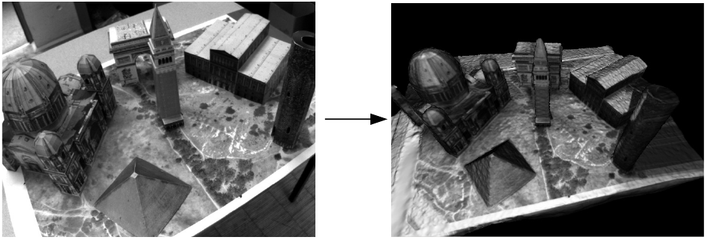
\includegraphics[width=0.8\textwidth]{live-cam}
    \caption{Dense 3D reconstruction. Left: camera input; right: reconstruction. Adapted from~\cite{livecam}}
    \label{fig:slam:example}
  \end{center}
\end{figure}

\section{Simultaneous localization and mapping}
Environment reconstruction has been receiving a lot of attention from the research  community, specially using Simultaneous Localization and Mapping (SLAM) procedures. 
Can be categorized according to the problem methodology in Extended Kalman filters, graph-based optimization and particle filters~\cite{Thrun2008_SLAM}.
The first work that used an incremental map building was done by \citeauthor{smith1990estimating}~\cite{smith1990estimating}, where the authors used Extended Kalman Filters (EKF) to recursively estimate a vector that includes the location of the sensing entity and feature elements of the environment. The uncertainty of the elements is modelled using probability density functions. Disadvantages of this approach is that the EKF procedure my be thrown off by incorrect measurements and it's limited to few landmarks.

The first solution using a graph-based optimization technique was presented by \citeauthor{lu1997globally}~\cite{lu1997globally}. The position of the entity and landmarks in the environment are represented as nodes in a graph. As the robot moves or senses landmarks, it adds nodes which are connected by arcs. Consecutive locations are tied together and landmarks are associated to the locations they were sensed in. If the graph is seen as a mass-spring system, the solution comes from the minimal energy state of the system. The main disadvantage of this methodology is that most implementations use off-line optimization of the graph, but it's able to keep track of up to $10^8$ landmarks~\cite{Thrun2008_SLAM}. 

The third common approach to the SLAM problem is using particle filters, it was first introduced by \citeauthor{montemerlo2002fastslam}~\cite{montemerlo2002fastslam}. Each particle is thought of as a guess for the trajectory of the entity in the environment. These particles are generated and, if degraded, re-sampled. An issue that has been noted for this method is that the complexity depends on the number of particles and the number of landmarks, this leads to a huge representation of the mapping; and there is no way of knowing how many particles are needed. 

A classification can be made by the nature of the sensing devices. While the SLAM problem with depth data may be considered closed, solving it with visual input alone is still an open research question. Furthermore, achieving a solution with spiking neural networks has received little attention despite the efficiency that this approach could provide. Most SLAM solutions only handle static indoor environments, although the vast majority of the world is outdoors and inherently dynamic. Another open question is how to deal with continuously accumulating sensing and/or inference errors, the recovery from which is key for dealing with ever-changing environments. 
%Papers that summarize and explain the mathematical framework of the SLAM problem can be found in the references chapter~\cite{Thrun2008_SLAM,Fuentes-Pacheco2012-slam,durrant2006simultaneous,bailey2006simultaneous}. 

In terms of sensor input, a division of SLAM that uses visual information as the sole external input is, not surprisingly, called \emph{visualSLAM}. In that group of algorithms  there are some that use a single camera, binocular vision, DVS, or RGB-D cameras, to name a few (Figure~\ref{fig:slam:camera-comparison}). 

A conventional camera captures colour information available for a fixed period of time (i.e. a frame). An RGB-D camera captures both colour and depth information; the latter is usually done with laser radars or structured light. A DVS is a visual sensor that emits an event whenever (i.e. dynamically) a pixel senses a change in contrast over time. A benefit of this is that static objects in a scene have a low probability of generating an event.
%The latter is not using only visual information, but it is using just a camera. 

\begin{figure}[h]
  \begin{center}
    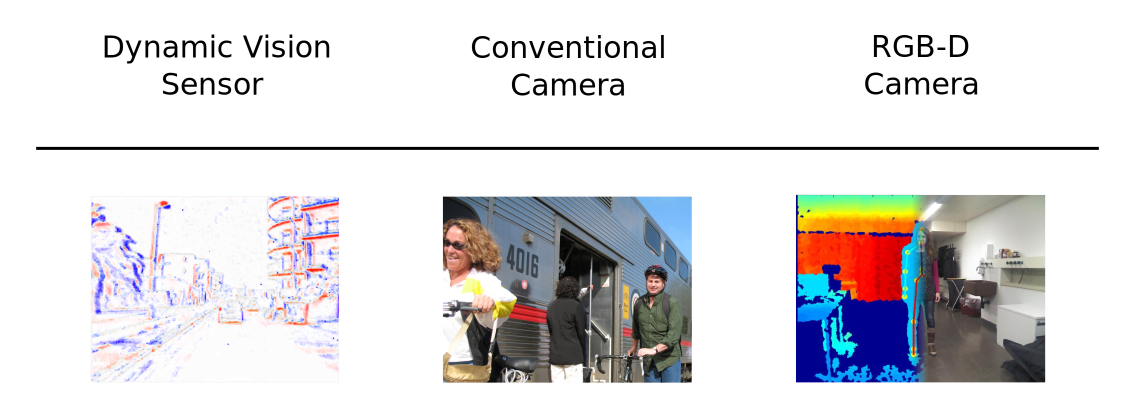
\includegraphics[width=\textwidth]{camera-comparison}
    \caption{Comparison of different visual inputs. Left: a DVS sensor, captures temporal contrast changes in a $\mu s$ scale (red and blue colours). Middle: a conventional camera captures light accumulated during a time window. Right: an RGB-D camera provides depth (left half of the sample image) plus colour (right half) information of a scene.}
    \label{fig:slam:camera-comparison}
  \end{center}
\end{figure}


If only images are used, the correspondence problem arises; where is a feature from one frame located in the next. To solve this, there are mainly two efficient approaches: the first is to use descriptors~\cite{lowe1999object,bay2006surf,alahi2012freak} (i.e. salient features of objects) or to use landmarks~\cite{sola2012impact,frintrop2006attentional} (i.e. full objects, often artificial). In our approach, the use of visual landmarks is chosen due to neural networks' image recognition capabilities. 

The algorithm known as \emph{MonoSLAM}~\cite{davison2007monoslam}, was the first to solve the SLAM problem in real time with a single camera. It is able to perform at 30 frames per second and considers both position and orientation of the camera. The limitations of this work is that is confined to indoor environments and it models motion with constant velocities.

%Spiking neural networks (SNN) need to convert any visual input to spike trains. 
\emph{Event-based 3D SLAM}~\cite{Weikersdorfer2014} is a work that uses a DVS  with RGB-D camera to create a sparse representation of 3D frames. It then uses Bayesian network and condensation particle filter algorithm. They obtain good results with few resources, but they are not using ANNs.

\citeauthor{villaverde2006morphological}~\cite{villaverde2006morphological} report a neural network approach for solving the localization and mapping. An interesting point is the use of Morphological Associative Memories (MAM), which are a type of content-addressable memory that uses morphological operations (dilation and erosion). In the learning and retrieval stages, MAMs utilize sums instead of products, and minimum (erosion) or maximums (dilation) instead of sums for vector and matrix operations. The main advantage to use MAMs is that they can store and recall morphologically strong-independent patterns, which have been proven to be robust against noise. 

Neural networks have also been used to complement other SLAM solutions, for instance by using a NN to better estimate the mapping in presence of noise and errors~\cite{choi2007neural}. A one hidden layer perceptron is used to estimate the uncertainty of the model and increase its accuracy. Another interesting NN extension to SLAM algorithms was reported by \citeauthor{saeedi2011neural}~\cite{saeedi2011neural}, they use a neural network to fuse the results of SLAM algorithms performed by multiple robots. The NN cluster representations into an occupancy grid map.

Hippocampus-based navigation studies has been developed by the neuroscience community. A simulation of a model of place cells is tested in a small robot through neural networks~\cite{burgess1997robotic}, with good results in terms of self-localization and environment recognition. A review of the different aspects of the theory behind hippocampus navigation was published by \citeauthor{sunderhauf2010learning}~\cite{sunderhauf2010learning}. 

A bio-inspired algorithm to solve the SLAM problem is \emph{RatSLAM}, it's based on the hippocampus of rodents, which has been studied for its involvement in navigation tasks. Pose is estimated by activity of place cells arranged in a competitive attractor neural network. If visual information is familiar with respect to a place cell, the latter gets excitatory input. Odometry helps select current active place cells. Results in semi-Cartesian space, on-line incremental, distributed representation via place cells~\cite{rat-slam,milford2008robot}.


\section{Proposal}
Our approach to solve the SLAM problem is to use spiking neural networks for their efficiency and biological plausibility. The primary external sensor would be visual, either a conventional camera or a dynamic vision sensor. The information from the sensor would then be scanned for landmarks (e.g. a lamp, door, tree, stop sign). To infer the position of the viewer, we will look for inspiration on published work that uses hippocampus models as that organ is known to be a basic component for navigational tasks in animals (see Section~\ref{sec:brain:hippo}). A link from visual information to the structure created through the neural network will have to be developed; from this link, a full 3D reconstruction should be available.\\

The milestones of this project are:
\begin{enumerate}
  \item Landmark identification and recognition through spike-based visual input. The initial task would be to develop an on-line learning neural network, the latter would then be modified for identification and recognition tasks.
  \item Tracking of landmarks. Adapt the network from the previous step to be able to provide information of where the landmarks are; this might include some attention modulation for moving objects.
  \item Localization estimation and depth perception. From the information provided by the tracking network (and possibly other sensors), feed another part of a larger network that will estimate the localization of the viewer. A result from this estimation would be the ability to perceive the distance of objects in the scene. 
  \item Mapping and reconstruction. The mapping problem will be solved in parallel to the localization one. For reconstruction a way to connect acquired visual information (i.e. video frames) to the estimated structure in the neural network will be developed and, thus, a full 3D reconstruction achieved.
\end{enumerate}


\section{Conclusions}
A complete model the visual cortex remains an open research question. Though many neural networks and computer vision models account for single visual functions, a unified solution has not been developed. Since environment reconstruction makes use of many of these functions, this research could lead to contributions to a general theory of vision. 

A hierarchical neural networks approach promises to have better results. The training of deep spiking neural networks is still in early stages of research, which brings another opportunity for contributions to neuroscience. Recurrent neural networks could provide the necessary framework to solve the training problem.


  \chapter{From video to spikes}
  \label{chp:img2spk}
  \section{Introduction}
\section{Dataset creation}
\section{Classification algorithms}
\section{SpiNNaker implementation}
\section{Results}
\section{Conclusions}

  \chapter{Conclusions}
  \label{chp:conclusions}
  \section{Conclusion}
\section{Further work}
\section{Plans for second and third year}

  \printbibliography


\end{document}
